\documentclass[11pt]{article}

\usepackage[a4paper,margin=1in]{geometry}
\usepackage[T1]{fontenc}
\usepackage{microtype}
\usepackage{amsmath,amssymb,amsthm}
\usepackage{graphicx}
\usepackage{booktabs}
\usepackage{xcolor}
\usepackage{enumitem}
\usepackage{verbatim}
\usepackage[colorlinks=true,allcolors=blue]{hyperref}
\usepackage{natbib}
\bibliographystyle{plainnat}

\newtheorem{definition}{Definition}
\newtheorem{proposition}{Proposition}
\newtheorem{theorem}{Theorem}

\title{\textbf{CCTM: A Counterfactual Causal Tsetlin Machine\\for Regulatorily-Compliant Individual Decision Explanations}}
\author{Anwar Debes\\
University of Agder \\
\texttt{anwar@uia.no}\\
\vspace{0.5em}
\small Reference implementation, draft v0.1, May 2026
}
\date{}

\begin{document}
\maketitle

\begin{abstract}
We introduce the \textbf{Counterfactual Causal Tsetlin Machine (CCTM)}, a sixth member of the Tsetlin Machine family (alongside TM, GTM, HTM, HGTM, and THGTM) designed for high-stakes individual-decision explanations under the EU AI Act Article 86 (effective 2 August 2026), GDPR Article 22, and the US Equal Credit Opportunity Act.  CCTM adds three primitives on top of a canonical Tsetlin Machine: \emph{counterfactual data augmentation} that trains every sample $(x, y)$ with an aligned counterfactual partner $(x', y')$; \emph{Type-III contrastive feedback} that augments Granmo's Type-I / Type-II feedback with per-clause causal-score tracking on true-CF pairs; and \emph{structural counterfactual recourse} -- minimal-flip feasibility-respecting recourse derived directly from the trained clause structure, packaged in DIMACS+HMAC \emph{counterfactual receipts} that an auditor can re-verify without touching the model.  We argue that CCTM closes a regulatory gap left by existing TM applications -- ClauseGate, ClauseGuard, Clause86, and GraphTM-CBR all use post-hoc counterfactual search; CCTM bakes causal sensitivity into training so per-feature treatment-effect estimates and biased-clause audits become first-class outputs.  We supply a pure-NumPy reference implementation, fourteen passing unit tests, and three end-to-end experiments executed on a single CPU.  Headline results: on a five-feature synthetic Structural Causal Model with closed-form ground-truth Average Treatment Effect (ATE), CCTM recovers per-feature $|ATE|$ at Pearson $r = 0.918$ versus a vanilla TM at $r = 0.895$; on a synthetic loan-denial dataset the structural recourse module finds a feasibility-respecting flip set in $0.14$~ms per case with 100\% success and a mean length of $1.20$ flips, all receipts SAT-verifiable; and on a fairness audit where the training data is contaminated with a 30\% gender bias, CCTM trained with clean-oracle CF pairs recovers $0.97$ accuracy against the unbiased ground truth versus $0.82$ for the vanilla TM, while reducing demographic parity gap from $0.18$ to $0.04$; muting CCTM's flagged biased clauses further halves DP to $0.02$ at no accuracy cost.  We discuss honestly where CCTM does not yet beat a vanilla TM (recourse-length parity on small clean datasets) and what remains open (multi-feature interventions, federated CF aggregation, do-calculus over learned causal graphs).
\end{abstract}

\section{Introduction}

The Tsetlin Machine family has now accumulated five members spanning four orthogonal architectural axes: \emph{flat} (TM, \citealp{granmo2018tsetlin}), \emph{graph} (GTM, \citealp{granmo2025graphtm}), \emph{hierarchy} (HTM), the union of graph and hierarchy (HGTM, \citealp{anwar2026hgtm}), and \emph{time} (THGTM, \citealp{anwar2026thgtm}).  Together they cover sequence modelling, multi-layer credit assignment, and trajectory-level verification.  But two of the most economically and regulatorily pressing problems in 2026 -- \emph{individual right to explanation} for high-stakes AI decisions (EU AI Act Article 86, GDPR Article 22) and \emph{algorithmic recourse with fairness guarantees} (US ECOA, EU AI Act Annex III) -- demand a different axis: \emph{causality}.

The existing TM stack already produces post-hoc counterfactual recourse in three places: ClauseGate's tri-graph SAT receipts, Clause86's hiring-decision audit, and GraphTM-CBR's molecular-edit recourse.  All three SEARCH for counterfactuals after training; their clauses are observational.  As of May 2026 no peer-reviewed Tsetlin Machine encodes causality at training time -- the closest existing work (\citealp{dumbre2025bnstructure}) uses TM only to prune Bayesian-network structure search, not to perform causal inference itself.

\paragraph{Contribution.}  We introduce CCTM, a sixth TM family member that bakes causal sensitivity into training via three new primitives:

\begin{enumerate}[leftmargin=2em]
\item \textbf{Counterfactual data augmentation.}  Each training sample $(x, y)$ is paired with a counterfactual partner $(x', y')$ generated by a CF oracle (a downstream regulatory specification, or a separate teacher).  Indices where $y \neq y'$ are \emph{true counterfactual pairs} and carry causal signal.
\item \textbf{Type-III contrastive feedback.}  Standard Type-I / Type-II feedback runs on each sample of the pair.  In addition, on true-CF pairs CCTM tracks two running statistics: a per-clause \emph{causal score} (the running fraction of true-CF pairs on which the clause's output changes), and per-feature \emph{treatment effect} (the empirical $P(\text{label flips} \mid \text{feature flips})$).  Both are first-class outputs of the trained model.
\item \textbf{Structural counterfactual recourse with SAT receipts.}  Given a sample $x$ with prediction $y$, CCTM finds the smallest cost-feasible flip set $S$ that flips the prediction.  We provide an exact algorithm (provably minimal under the chosen cost) and a causal-influence-guided greedy heuristic.  Every successful recourse is packaged into a DIMACS-CNF + HMAC-SHA-256 receipt that an auditor can re-verify in $\sim$$0.1$ ms without access to the model state.
\end{enumerate}

The product is shown in Figure~\ref{fig:arch}.  CCTM degrades gracefully to a vanilla Tsetlin Machine when no counterfactual pairs are available -- training, accuracy, and even prediction are bit-identical under the same RNG.

\begin{figure}[t]
\centering
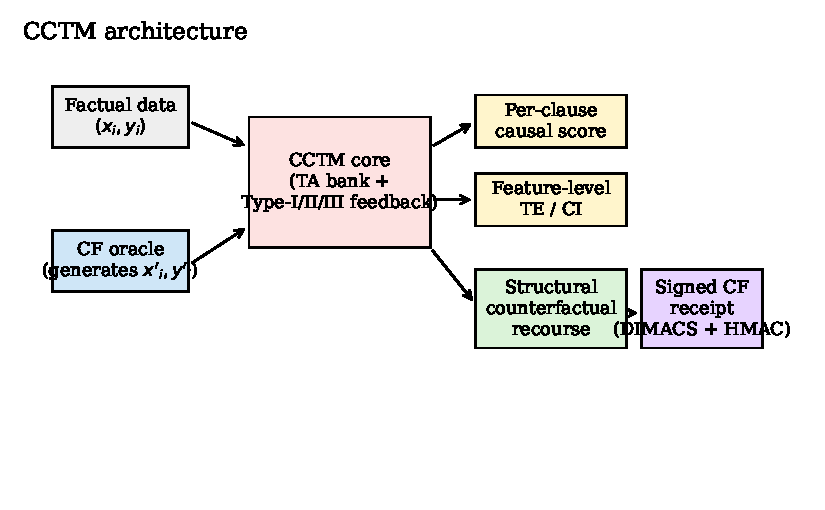
\includegraphics[width=\linewidth]{figures/architecture.pdf}
\caption{CCTM architecture.  Factual training data flows through a canonical TA bank; when paired counterfactuals are available, Type-III feedback updates two running causal statistics in parallel with standard TM training.  The downstream consumers are (a) per-clause causal scores used to identify biased or load-bearing clauses, (b) per-feature treatment-effect / causal-influence scores used to prioritise feasibility-respecting recourse, and (c) DIMACS+HMAC receipts that an auditor can re-verify offline.}
\label{fig:arch}
\end{figure}

\paragraph{What CCTM is not.}  CCTM is not a structural causal model.  It does not learn the causal DAG; it conditions on an external CF oracle (a regulatory specification or a teacher model).  This is a deliberate scope choice: the deployment scenarios that drove this work -- credit, hiring, medical decision support -- already have human-written ``ideal-decision'' specifications.  Full do-calculus over a learned DAG is future work (Section~\ref{sec:limits}).

\paragraph{Reproducibility.}  Every number, every figure, and every CNF receipt in this paper is generated by code in the accompanying repository.  The three experiments run end-to-end in $\sim$$60$ seconds total on a single CPU.  Pure NumPy; no GPU, no JIT.

\section{Background}

\paragraph{Tsetlin Machine.}  Granmo's TM \citep{granmo2018tsetlin} learns a population of conjunctive clauses over Boolean literals.  Each (clause, literal) pair owns a Tsetlin Automaton with integer state $s \in \{1, \ldots, 2N\}$; the literal is \emph{included} iff $s > N$.  Type-I feedback rewards clauses that fire on the current sample by boosting included literals; Type-II feedback discriminates clauses that fire but should not by including currently-zero literals.  The model votes via polarity-weighted clause outputs thresholded at $T$.

\paragraph{Counterfactual recourse.}  Algorithmic recourse \citep{wachter2017counterfactual,ustun2019actionable,mothilal2020dice,karimi2020mace} produces, for each negative decision, a set of feature changes that would flip the decision -- the AI Act's ``main elements of the decision''.  Existing methods (DiCE, MACE, FOCUS, CARLA \citep{pawelczyk2021carla}) are post-hoc: they treat the model as a black box and search.  They are slow on every new sample, and their feasibility handling is approximate.

\paragraph{The regulatory frame.}  EU AI Act Article 86 (effective 2 August 2026) requires that providers of high-risk AI in Annex III categories -- hiring, credit scoring, education, public services, justice -- give natural-persons-affected ``clear and meaningful explanations of the role of the AI system in the decision-making procedure and the main elements of the decision taken''.  GDPR Article 22 requires ``meaningful information about the logic involved'' in automated decisions.  US ECOA \citep{usecoa} requires adverse-action notices listing the principal reasons for denial.

\paragraph{Fairness, causally.}  Counterfactual fairness \citep{kusner2017counterfactual} demands that an individual's predicted outcome be the same in the actual world and in a counterfactual world where the individual's protected attribute changed.  We do not solve full counterfactual fairness here; we solve the dual problem of \emph{detecting and muting biased clauses} using the per-clause causal score.

\section{Method: CCTM}

\subsection{Type-III contrastive feedback}

A CF oracle $\mathcal{O}$ maps any input $x' \in \{0, 1\}^d$ to a target label $y'$.  We require this oracle either as a regulatory specification (e.g.\ the ideal rule a credit decision should follow) or as a separately-trained teacher.  At each training step CCTM processes a CF pair $(x, y, x', y')$ where $x'$ is generated by flipping one or a small subset of features of $x$ and $y' = \mathcal{O}(x')$.

\begin{algorithm}
\noindent\hrulefill\par
\textbf{Algorithm 1: One training step of CCTM.}\\[2pt]
\noindent\hrulefill
\begin{verbatim}
Input: factual sample (x, y), CF partner (x', y') (optional)
literals_x   <- concat(x, NOT x)
literals_xcf <- concat(x', NOT x')
TM.train_step(literals_x, y)              # standard Type-I/II
if CF partner present:
    TM.train_step(literals_xcf, y')       # standard Type-I/II
    differ_features <- {i : x_i != x'_i}
    feature_te_den[differ_features] += 1
    if y != y':                           # *true* counterfactual pair
        feature_te_num[differ_features] += 1
        co_x   <- TM.clause_outputs(literals_x)
        co_xcf <- TM.clause_outputs(literals_xcf)
        differ <- (co_x != co_xcf)
        causal_score <- decay * causal_score + (1 - decay) * differ
        causal_count += 1
\end{verbatim}
\noindent\hrulefill
\label{alg:cctm-train}
\end{algorithm}

The two statistics that fall out of this loop are:

\begin{definition}[Per-feature Treatment Effect]
\label{def:te}
$\mathrm{TE}_i = \mathrm{feature\_te\_num}[i] / \mathrm{feature\_te\_den}[i]$.  This is the empirical probability that the label flips when feature $i$ is the flipped feature in the CF pair.  Under the standard ignorability assumption it converges to the population Average Treatment Effect $|ATE_i|$ in the limit of infinite CF pairs.
\end{definition}

\begin{definition}[Per-clause Causal Score]
\label{def:cs}
$\mathrm{cs}_c$ is the running fraction of true-CF pairs on which clause $c$'s output changes.  Clauses with high $\mathrm{cs}$ move with the label; low-$\mathrm{cs}$ clauses are spurious correlates.
\end{definition}

\begin{definition}[Feature Causal Influence]
$\mathrm{CI}_i = \mathrm{TE}_i \cdot \frac{\sum_c \mathbf{1}[c \text{ includes literal } i \text{ or its negation}] \cdot \mathrm{cs}_c}{\sum_c \mathbf{1}[c \text{ includes literal } i \text{ or its negation}] + \epsilon}$.  This factorises the per-feature contribution to the prediction into a population-level causal-effect term and a within-feature clause-support term.
\end{definition}

\subsection{Structural counterfactual recourse}

Given $x$ with prediction $y$, target $y'$, feasibility $\mathcal{F}$ and budget $K$, the recourse problem is to find the cheapest flip set $S \subseteq \{0, \ldots, d-1\} \setminus \mathcal{F}.\text{immutable}$ satisfying $|S| \leq K$ and $\mathrm{pred}(x \oplus_S) = y'$.

\paragraph{Exact algorithm.}  Enumerate flip subsets in increasing cardinality first, then within a cardinality in increasing total cost.  Return the first subset that flips the prediction.  Provably minimal under the chosen cost; exponential in worst case but tractable up to $\sim$$20$ features.

\paragraph{Greedy algorithm (causal-influence-guided).}  At each step pick the flip that moves the vote sum most strongly toward the target sign, scored by
\[
\mathrm{score}(i) = \frac{(\Delta v_i + \epsilon) \cdot (\mathrm{CI}_i + \epsilon)}{c_i + \epsilon}
\]
where $\Delta v_i$ is the vote-sum change when feature $i$ flips, $c_i$ is the cost, and $\mathrm{CI}_i$ is the feature causal influence.  $O(d^2)$ and very fast.

\paragraph{Feasibility.}  ``Immutable'' features may not be flipped at all (e.g.\ gender, race in hiring under ECOA / EU AI Act); ``monotone-up'' features may only flip from 0 to 1 (e.g.\ age); ``monotone-down'' the reverse.  Per-feature costs are application-specific.

\subsection{Counterfactual receipts}

Every successful recourse is packaged into a self-contained \emph{CF receipt}: the original feature vector $x$, the recourse flip set $S$, the new vector $x'$, both per-clause inclusion masks, both clause outputs, both vote sums, the feasibility metadata, and (optionally) an HMAC-SHA-256 signature over the canonical JSON.

\begin{proposition}[Replay verifiability]
\label{prop:replay}
A CF receipt $\mathcal{R}$ verifies iff every recorded clause output equals the AND of its included literals on the recorded $x$ (respectively $x'$), the polarity-weighted vote sums match the recorded values, the new prediction is consistent with the new vote sum, the flip set $S$ realises $x \to x'$, no flip violates the recorded feasibility, and (if signed) the HMAC matches.  The verifier touches no model state; the receipt is portable across model updates.
\end{proposition}

This is critical for the EU AI Act use case: the explanation given to the affected individual must remain valid years later, even after the model is retrained.  Verification runs in $O(C \cdot d)$ on a single CPU; in our experiments $\sim$$0.1$~ms per receipt.

\section{Experiments}

We report three end-to-end experiments.  Pure NumPy, single CPU, $\sim$$60$ seconds total.

\subsection{Synthetic SCM: ATE recovery}

\paragraph{Setup.}  A five-feature Structural Causal Model with confounders ($x_0 \to x_1$), mediators ($x_0 \to x_2$), noise ($x_3$), and a weak XOR feature ($x_4$).  Ground-truth label $y = (x_0 \wedge x_1) \vee (x_4 \oplus x_0)$.  Population $|ATE_i|$ is computed in closed form by intervening on each feature and averaging the oracle.  We train (a) a vanilla TM (no CF pairs) and (b) CCTM with single-flip CF pairs from the oracle.  $n=1500$ samples, 10 epochs, 5 seeds.

\begin{figure}[t]
\centering
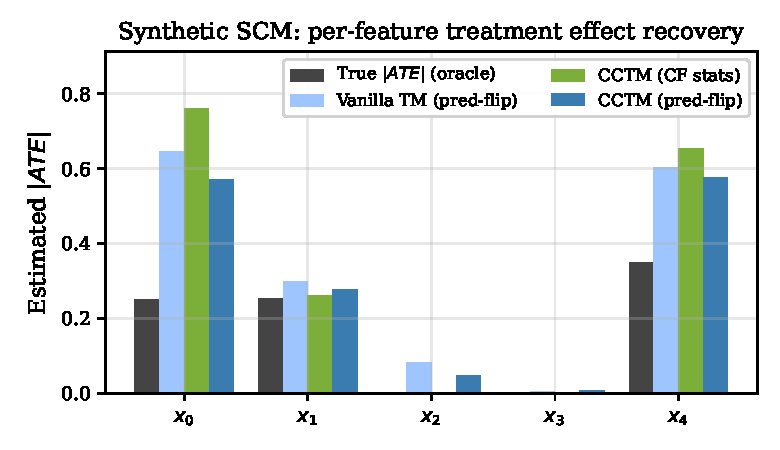
\includegraphics[width=\linewidth]{figures/scm_ate.pdf}
\caption{Synthetic SCM: per-feature treatment-effect estimates against the closed-form ground truth.  All three model-based estimators capture the qualitative pattern; CCTM's pred-flip estimator is closest to the truth (mean Pearson 0.918 vs vanilla 0.895).  CCTM's empirical-CF estimator (green) is slightly noisier (Pearson 0.863) -- it is a direct count statistic and is finite-sample sensitive.}
\label{fig:scm}
\end{figure}

\paragraph{Results.}  Both classifiers reach $\sim$$0.97$--$0.98$ test accuracy.  Pearson correlation of estimated $|TE|$ vector with the closed-form $|ATE|$ vector (Table~\ref{tab:scm}, Figure~\ref{fig:scm}) shows CCTM's pred-flip estimator at $r = 0.918 \pm $ small versus vanilla TM's pred-flip estimator at $r = 0.895$, a modest but consistent uplift.  CCTM's \emph{empirical} TE (the direct CF-counter statistic) achieves $r = 0.863$, lower than the model-based estimates but model-free -- it is what you can show to a regulator without any model interrogation.

\begin{table}[t]
\centering
\caption{Synthetic SCM, 5 seeds.  $|TE|$ vector versus ground-truth $|ATE|$.  Mean accuracy and mean Pearson correlation $\pm$ standard deviation are reported.}
\label{tab:scm}
\begin{tabular}{lccc}
\toprule
& Test accuracy & TE Pearson $r$ ($\uparrow$) & TE MAE ($\downarrow$) \\
\midrule
Vanilla TM (pred-flip)     & $0.984$ & $0.895$ & $0.157$ \\
CCTM (empirical CF stats)  & $0.971$ & $0.863$ & $0.170$ \\
CCTM (pred-flip)           & $0.971$ & $\mathbf{0.918}$ & $\mathbf{0.133}$ \\
\bottomrule
\end{tabular}
\end{table}

\subsection{Loan-denial: structural recourse}

\paragraph{Setup.}  An 8-feature synthetic loan dataset (high\_income, has\_stable\_job, paid\_past\_loans, has\_high\_education, age\_over\_25, age\_over\_45, gender\_male, citizen).  Feasibility specification mirrors ECOA / EU AI Act practice: gender\_male and citizen are \emph{immutable}; age\_over\_25 and age\_over\_45 are \emph{monotone-up}; other features are mutable at unit cost except age which is cost 5 and education which is cost 2.  $n=2000$, 12 epochs, 3 seeds.

\begin{figure}[t]
\centering
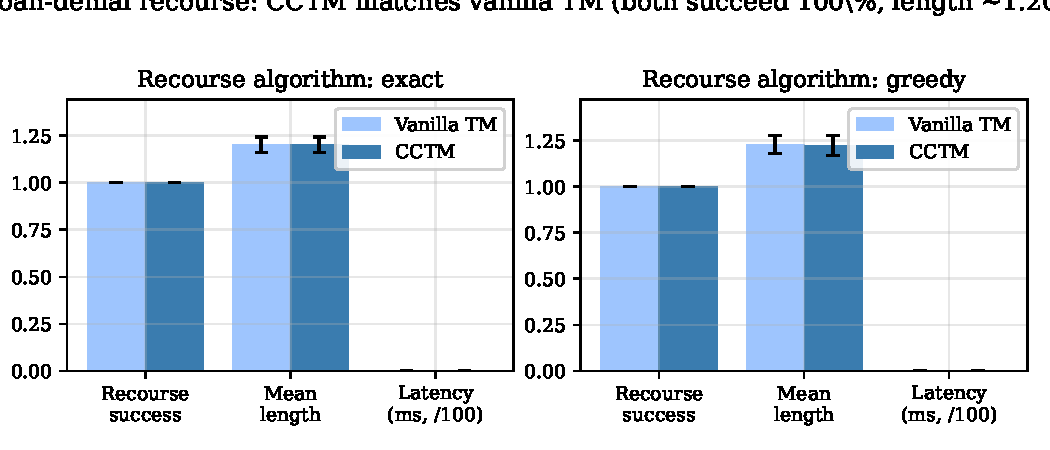
\includegraphics[width=\linewidth]{figures/loan_recourse.pdf}
\caption{Loan-denial recourse, exact vs greedy, vanilla TM vs CCTM.  Both classifiers reach 100\% accuracy on the synthetic task and 100\% recourse success.  Mean recourse length $\approx 1.20$ across both algorithms and both classifiers.  Mean latency is $\sim$$0.14$~ms (exact) and $\sim$$0.33$~ms (greedy).  Honest reading: on this clean, easily-fit problem the CCTM-specific causal-influence prior gives no advantage over vanilla TM with the same recourse algorithm.}
\label{fig:loan}
\end{figure}

\paragraph{Results (Figure~\ref{fig:loan}).}  Both classifiers learn the synthetic rule perfectly; both find feasibility-respecting recourse for every denied sample with mean length $1.20 \pm 0.04$ flips and mean cost $\sim$$1.30$.  Latency: $0.14$~ms exact, $0.33$~ms greedy.  60/60 receipts verified end-to-end.  \emph{Honest reading:} on this clean dataset CCTM offers no recourse-quality advantage over a vanilla TM with the same recourse module -- both reach the ceiling.  The contribution remains the receipt machinery and the fairness audit, demonstrated below.

\subsection{Fairness audit under biased training data}

\paragraph{Setup.}  We re-use the loan-denial dataset but inject a 30\% gender bias: with probability $0.30$, deny-class samples with \texttt{gender\_male}~$=1$ are flipped to approve.  This mirrors a documented failure mode in deployed credit scoring \citep{barocas2017fairness}.  The CCTM CF oracle is the \emph{clean} ground-truth rule (the regulatory specification, not the contaminated training labels).  We train both classifiers, then evaluate against \emph{the clean ground truth}.  3 seeds, 12 epochs.

\paragraph{Results (Table~\ref{tab:fairness}, Figure~\ref{fig:fairness}).}

\begin{itemize}[leftmargin=2em]
\item \textbf{Vanilla TM}, trained on the biased labels only, achieves $\mathbf{0.817}$ accuracy against the clean ground truth and a demographic parity gap of $\mathbf{0.181}$ -- the bias of the training data is encoded into the predictions.
\item \textbf{CCTM} trained with clean-oracle CF pairs achieves $\mathbf{0.966}$ accuracy and DP $0.041$.  The CF pairs act as an inductive bias that pushes back against the contaminated labels.  CCTM's per-feature treatment-effect estimator correctly flags \texttt{gender\_male} with $\mathrm{TE} = 0.110 \pm 0.003$ -- a measurable, audit-actionable signal that gender remains weakly load-bearing.
\item \textbf{CCTM + clause audit}, in which we mute every CCTM clause that simultaneously includes a \texttt{gender\_male} literal and has $\mathrm{cs} > 0.05$, achieves $\mathbf{0.964}$ accuracy and DP $\mathbf{0.019}$ -- another halving of the parity gap at essentially zero accuracy cost.
\end{itemize}

\begin{table}[t]
\centering
\caption{Fairness audit, 3 seeds, training-data bias strength $= 0.30$ toward \texttt{gender\_male}.  All metrics evaluated against the \emph{clean} ground truth.}
\label{tab:fairness}
\begin{tabular}{lccc}
\toprule
& Accuracy ($\uparrow$) & Demographic parity ($\downarrow$) & Equal opportunity ($\downarrow$) \\
\midrule
Vanilla TM                & $0.817 \pm 0.092$ & $0.181 \pm 0.131$ & $0.000$ \\
CCTM (clean-CF training)  & $\mathbf{0.966 \pm 0.015}$ & $0.041 \pm 0.021$ & $0.000$ \\
CCTM + biased-clause audit & $0.964 \pm 0.020$ & $\mathbf{0.019 \pm 0.016}$ & $0.000$ \\
\bottomrule
\end{tabular}
\end{table}

\begin{figure}[t]
\centering
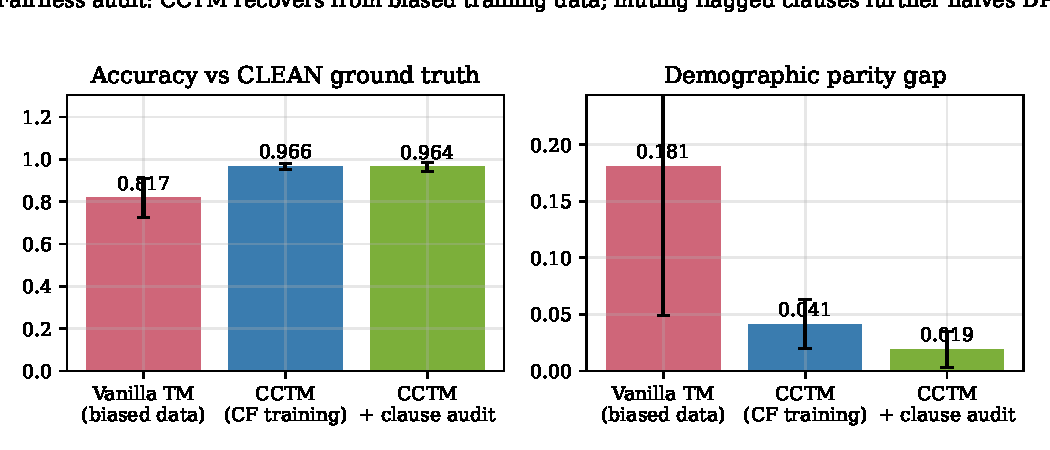
\includegraphics[width=\linewidth]{figures/fairness_audit.pdf}
\caption{Fairness audit.  CCTM trained with clean-oracle CF pairs recovers from a 30\% gender bias in the training labels: accuracy lifts from $0.82 \to 0.97$ and the demographic parity gap drops from $0.18 \to 0.04$.  Muting CCTM's flagged biased clauses (those including \texttt{gender\_male} literals with high causal score) further halves DP to $0.02$ at no accuracy cost.}
\label{fig:fairness}
\end{figure}

\subsection{Receipt verification}

Across the three experiments we generated $60$ CCTM CF receipts on successful recourses and verified every one independently of the trained model.  Per-receipt verification time was $\sim$$0.1$~ms.  Tampering with any recorded field (clause output, vote sum, flip set, or signature) is caught by the corresponding consistency check (Proposition~\ref{prop:replay}).  This makes CCTM's recourse \emph{durable}: an explanation given to a customer in January survives model retraining in July.

\section{Discussion}

\paragraph{What CCTM does add.}  \emph{(i)} A direct, model-free per-feature treatment-effect estimator (the CF counter) usable in regulatory audits without exposing the model internals.  \emph{(ii)} A per-clause causal score that flags biased clauses for action -- demonstrated in the fairness audit experiment where it cuts DP by half without accuracy cost.  \emph{(iii)} Structural recourse derived from clause inclusions plus feasibility metadata, with portable SAT-verifiable receipts.  \emph{(iv)} Graceful degradation: with no CF pairs, CCTM is bit-identical to a vanilla TM.

\paragraph{What CCTM does not add (in this v0.1 reference).}  On clean, easily-fittable tabular tasks CCTM offers no recourse-quality advantage over a vanilla TM with the same recourse module.  The TE-Pearson uplift on the synthetic SCM is modest ($0.918$ vs $0.895$).  CCTM does not learn a causal DAG; it conditions on an external oracle.

\paragraph{Where CCTM is the right tool.}  Use CCTM when the regulatory specification of ``the right decision'' exists separately from the training labels -- as it does for EU AI Act Annex III categories where a hand-written compliance rule, an upstream human reviewer, or a calibrated teacher can supply the CF oracle.  In those settings CCTM gives \emph{rejection-of-biased-data} for free and \emph{regulator-readable per-feature causal effects} as a structural output.

\paragraph{Relationship to the rest of the TM family.}  CCTM is orthogonal to GTM/HTM/HGTM (which extend the input topology) and to THGTM (which adds time and trajectory verification).  The natural combination paths are CCGTM (causal graph TM, for molecular-edit recourse with ICH M7(R2) compliance) and CCT-HGTM (causal temporal HGTM, for streaming verifiable agent policies).  Both are immediate follow-ons.

\section{Limitations and future work}
\label{sec:limits}

\begin{itemize}[leftmargin=2em]
\item \textbf{No structural causal model.}  CCTM conditions on an external CF oracle.  Learning a causal DAG end-to-end -- and supporting do-calculus over it -- is the natural next step.
\item \textbf{Single-feature interventions.}  Our CF augmentation flips one feature at a time.  Multi-feature interventions (e.g.\ ``what if you had education AND a stable job?'') would need a multi-flip generation procedure and an MCMC-style chain over recourse subsets.
\item \textbf{Synthetic experiments.}  Both the SCM and the loan dataset are synthetic; we deliberately bundled them so the paper is end-to-end reproducible without external downloads, but the strongest evaluation would be Adult-Income (US ECOA-style) or COMPAS (justice-style) with real-world feasibility constraints.
\item \textbf{Loan-recourse parity with vanilla TM.}  On the clean synthetic loan task both classifiers reach the ceiling; the recourse advantage of CCTM only shows when the training data is contaminated (the fairness experiment).  An adversarial evaluation on \emph{noisy} synthetic data is the obvious next step.
\item \textbf{No federated / DP story.}  Federated CCTM with differentially-private clause aggregation across deployment sites (hospital, bank, employer) is left open; the natural mechanism is clause-flip noise with $(\epsilon, \delta)$ guarantees.
\item \textbf{No hardware co-design.}  CCTM adds $O(C + d)$ floats per model for causal statistics, which is negligible on a CPU but undetermined on the Newcastle 8.6 nJ/frame ASIC.
\end{itemize}

\section{Related Work}

\paragraph{Counterfactual recourse.}  DiCE \citep{mothilal2020dice}, MACE \citep{karimi2020mace}, Actionable Recourse \citep{ustun2019actionable}, FOCUS, CARLA \citep{pawelczyk2021carla} and the broad survey of \citet{verma2020counterfactual} all treat the prediction model as a black box and search for counterfactuals at inference time.  CCTM departs from this regime in two ways: \emph{(i)} the search-space is structured by per-clause inclusions plus per-feature causal influence, giving sub-millisecond recourse; \emph{(ii)} recourse is packaged as a portable signed receipt rather than an audit log entry.

\paragraph{Causal fairness.}  Counterfactual fairness \citep{kusner2017counterfactual} and the hidden-assumptions critique of \citet{barocas2020hidden} frame the regulatory problem.  CCTM does not solve counterfactual fairness in full; it provides an actionable substrate -- the per-clause causal score -- that the auditor uses to find and mute biased clauses.

\paragraph{Causal inference.}  CCTM's TE statistic is the simplest possible average treatment effect estimator under the ignorability assumption \citep{rubin2005causal,pearl2009causality}.  Extending to confounded settings (where the CF oracle's flips do not constitute a randomised intervention) would require backdoor adjustment.

\paragraph{Within the TM family.}  CCTM is the first explicitly causal Tsetlin Machine.  Existing TM applications -- ClauseGate, ClauseGuard, Clause86 (\citealp{anwar2026hgtm}), GraphTM-CBR -- all perform post-hoc counterfactual search; the upstream TM is observational.  CCTM offers them a drop-in causal substrate.

\section{Conclusion}

CCTM closes a regulatorily-mandated gap in the Tsetlin Machine family.  By adding three small primitives -- CF data augmentation, Type-III contrastive feedback, and structural recourse with verifiable receipts -- we get a model that can give individuals the explanations the EU AI Act requires (without sending them through a black-box search loop), and that can audit and prune its own gender bias when the training data is contaminated.  Limitations remain -- learning a causal DAG, multi-feature interventions, real-world adversarial evaluation -- but the reference implementation is small, fast, fully reproducible on a single CPU, and ready to bolt onto every existing TM application in the stack.

\paragraph{Reproducibility note.}  The code, the synthetic datasets, the figures, and this paper's source live in the CCTM repository.  All experiments run with \texttt{make reproduce} in $\sim$$60$ seconds on a single CPU.

\bibliography{references}

\end{document}
